\documentclass{mise_en_page}

\projet{Projet Ingéniérie}
\equipe{H4314}
\responsable{Pierre Lulé}
\redacteurs{Sébastien Laurent, Léo Lefebvre, Jérémy Tuloup} % Optionnel
\titre{Dossier de spécification technique des besoins du système}
\version{1.0}
\objet{Présenter les axes de progrès envisagés sur le système existant,
définir les exigences fonctionnelles et non fonctionnelles, de manière
à répondre aux besoins du clients et à l’appel d’offre.}
\etat{non validé} %draft, non relu, non validé, validé
\begin{document}

\maketitle

\tableofcontents

\newpage

\section{Introduction}
Ce document va exprimer l’ensemble des besoins techniques reliés au
nouveau système de monitoring à distance de la société COPEVUE. Il va
détailler les axes de progrès offert par le nouveau système. Les
exigences fonctionnelles et non fonctionnelles du système seront aussi
détaillées.

\section{Axes d’amélioration
retenus}
\subsection{Axes de progrès retenus}
\subsubsection{Réduire les déplacements humains coûteux et polluants}
Notre système doit être capable de traiter les données récupérées des
différents sites de manière à déterminer des solutions optimisées pour
plusieurs critères.

Ce traitement doit pouvoir, après un système d’aide à la décision
adapté, mettre en place des trajets pour les camionneurs et les
techniciens assurant la maintenance des sites de manière à réduire leur
impact écologique sur l’environnement, c’est à dire qu’ils doivent être
le plus court possible tout en desservant tous les sites concernés par
une maintenance évitant ainsi des aller-retours très polluants.

Cet axe de progrès est très important pour la préservation de
l’environnement et également pour une diminution des coûts de
déplacement et pour offrir un service optimal pour les différents
sites.

\subsubsection{Suivi temps réel}
La mise en place de notre système permettra un suivi constant en temps
réel de tous les sites isolés, peu importe leur position et les
difficultés rencontrées pour y accéder. Ceci constitue un axe de
progrès non négligeable. La solution actuelle nécessite des relevés
manuels réguliers, à une fréquence bien trop longue, et parfois non
respectée, pour garantir l’efficacité voir l’utilité de certains sites
(par exemple une station de réserve d’eau en cas d’incendie).

\subsection{Axes de progrès marginaux}
\subsubsection{Traçabilité des opérations et de l’état du système}
La mise en place d’un central chargé de collecter toutes les données en
temps réel permet à la fois d’établir un historique des différents
relevés, mais aussi de prévoir les opérations de maintenance à
effectuer. Toutes ces données informatiques peuvent en effet être
traitées intelligemment afin de mettre en place un suivi à long terme
de chacun des sites. Le fait de pouvoir prévoir les opérations de
maintenance permet de réduire les coûts liés à cette dernière (exemple
: déplacement préventif évitant des pertes matérielles, regroupement de
déplacements dans des secteurs proches et/ou planification dans des
horaires standards, etc.).

\section{Description des exigences non fonctionnelles de votre
futur système}
\subsection{Intégration de l’existant}
La solution doit s’intégrer aisément avec les différents acteurs du
projet. Notre système doit donc être adapté aux interventions des
agents de maintenance afin d’en assurer le suivi et la planification.
Ces opérateurs peuvent être externes au projet, ce pourquoi il faut
leur garantir un accès propre et sécurisé au système, de préférence
avec des appareils portables.

\subsection{Robustesse}
La répartition de ces sites isolés dans des milieux aux conditions
parfois extrêmes impose une robustesse infaillible du système. Il doit
donc être totalement résistant et maîtriser son environnement extérieur
(conditions climatiques, champs électromagnétiques, vandalisme et
détériorations, défaillances...) pouvant entraîner des redémarrages
intempestifs du système.

\subsection{Fiabilité}
La difficulté d’accès ainsi que les coûts engendrés par des déplacements
sur sites isolés impliquent une forte exigence au niveau de la
fiabilité. En effet, le système ne doit jamais se retrouver bloqué et,
de manière plus générale, nécessiter une opération de maintenance
logicielle manuelle (ce type d’opération étant prévue à distance par le
déploiement de mises à jour depuis le poste central).

\subsection{Évolutivité et maintenabilité}
La conception du système se veut générique dans l’objectif d’une
utilisation détachée du contexte. En satisfaisant cette exigence, il
sera aisé d’adapter le système à d’autres applications, en ne modifiant
que la configuration. De plus, le système doit pouvoir vérifier la
présence de mises à jour logicielles qui lui sont destinées et les
appliquer de manière totalement autonome tout en s’adaptant à la
configuration locale (matérielle et logicielle). Les extensions
matérielles sont cependant plus rares, mais leurs compatibilités
logicielles pourront être assurées soit par des mises à jour distantes,
soit manuellement par un agent de maintenance certifié.

\subsection{Limitations technologiques}
Le choix de certaines technologies et de matériels comme le GPS et GSM,
dont le fonctionnement interne est géré par des sociétés de
télécommunication, peut avoir quelques problèmes dans son utilisation.
Le système devra donc pouvoir s’adapter aux différentes situations
possibles engendrées par l’utilisation de ces technologies, notamment
dans un environnement à fort champ magnétique, pouvant troubler les
dispositifs de communication. Il faut également avoir conscience
d’éventuels problèmes liés aux opérateurs téléphoniques qui pourrait
subir des pannes matérielles.

\subsection{Généricité}
Notre système doit être développé de manière à ce qu’il puisse s’adapter
à des environnements de monitoring différents qui ne se limitent pas à
l’observation de cuves. Il lui faudra pour cela être paramétrable
rapidement et facilement pour s’interfacer avec d’autres systèmes (par
exemple pour surveillance des réservoirs d’eau dispersés sur un
territoire (forêt) servant à lutter contre les incendies, domotique).
Il convient donc d’avoir une approche de « progicialisation ».

Cela doit nous amener à une réflexion approfondie sur le paramétrage des
modules, de l’interface etc.

\subsection{Réutilisation et portabilité des composants}
La conception de notre système sera orientée de façon à autoriser la
réutilisation des composants sélectionnés dans d’autres applications
comme par exemple pour de la domotique ou dans d’autres domaines
demandant un système de maintenance avec un tel réseau de capteur.

Notre conception devra suivre également une optique selon laquelle les
composant utilisés par notre système soient utilisables pour plusieurs
environnements ayant des caractéristiques différentes (désert du Sahara
ou régions froides du nord de la Norvège).

\subsection{Ergonomie}
Ce sont des non informaticiens qui utiliseront notre futur système. On
définira les IHM en fonction de ces utilisateurs : sur site central
pour les acteurs de la télésurveillance, sur station
(Mobile/PDA/Smartphones) pour les intervenants sur site (camionneur,
propriétaire,…).

Ces IHM seront très intuitives, compréhensibles et facile à utiliser.

\subsection{Traçabilité}
Notre système devra garder une trace de toute intervention (distante ou
sur site). Ces traces devront être répertoriées pour une période de
minimum 2 ans. Elles permettront de remonter dans l’historique des
tâches pour connaître l’origine d’une éventuelle erreur, mais aussi
pour réaliser une analyse de données afin d’en dégager une prévision de
maintenances récurrentes.

\section{Description des exigences fonctionnelles de votre futur
système }
Nous allons dresser la liste des exigences fonctionnelles de notre futur
système :

\subsection{Acquisition de données}
Le système embarqué doit être capable de récupérer les données en
provenance de différents capteurs.

Exigences non fonctionnelles associées :

\begin{description}
\item[Fiabilité :] Il faut qu’au maximum un capteur tombe en panne chaque
année
\item[Robustesse :] On doit pouvoir remplacer un capteur ou couper et
réactiver son alimentation sans l’endommager
\item[Intégration de l’existant :] si possible, les capteurs existant
devraient être réutilisés
\item[Évolutivité et Maintenabilité :] l’acquisition ne doit pas être
dépendante d’un type de capteur
\item[Généricité :] les capteurs doivent être génériques et le système
doit pouvoir s’adapter à plusieurs types de capteurs génériques
\end{description}
\subsection{Localisation planétaire}
Le système embarqué doit entièrement être localisable sur la surface de
la planète

Exigences non fonctionnelles associées :

\begin{description}
\item[Fiabilité :] les systèmes de localisation intégrés aux véhicules
agents de maintenance doivent pouvoir êtres fiables même en cas
d’intempérie.
\item[Évolutivité et maintenabilité :] le système de localisation doit
pouvoir être remplacé séparément par une autre technologie en cas
exceptionnel.
\item[Limitations technologiques :] un dysfonctionnement d’une puce doit
pouvoir être détecté
\item[Ergonomie :] les systèmes de localisation doivent offrir
l’interface la plus simple aux agents de maintenance. La destination de
l’agent doit pouvoir être indiquée à distance au GPS sans que l’agent
n’ait de doutes sur sa destination.
\end{description}
\subsection{Communication avec le serveur central}
Le système embarqué doit communiquer avec le serveur central de manière
fiable et sans perte de données. Le système envoie périodiquement les
informations sur les différents capteurs en PUSH. La période d’envoi
des trames d’information est configurable à souhait (toutes les heures,
toutes les deux heures, tous les mois, …). Nous estimons cependant
qu’un envoi quotidien répond amplement aux besoins de chaque site. 

La transmission des données s’appuie sur le réseau GSM. en cas
d’indisponibilité du réseau, ou de non-couverture (pour des sites
implantés dans un environnement extrême), il sera possible d’utiliser
la communication par satellite.

Exigences non fonctionnelles associées : 

\begin{description}
\item[Fiabilité :] les données doivent être transmises sans perte. En cas
de coupure ou d’indisponibilité du réseau, les données sont stockées
sur la mémoire interne du système puis envoyées lorsque le réseau
redevient disponible.
\item[Robustesse :] la robustesse de la communication entre le système et
le serveur central repose principalement sur la qualité et la
robustesse des infrastructures déployées par l’opérateur de téléphonie.

\item[Limitations technologiques :] la transmission des données se fait
via le réseau téléphonique (GSM), réseau dont les infrastructures sont
maintenues déployées par les opérateurs téléphoniques. Dans le cas
d’une indisponibilité réseau, ou dans le cas où le site ne serait pas
couvert, la communication pourra se faire via satellite.  
\end{description}
\subsection{Transmission des informations des capteurs au système}
Toutes les informations doivent être mises à disposition de
l’utilisateur (et du serveur central) de manière simple et portable
(indépendamment de la plateforme utilisée).

Les capteurs sont reliés sur un réseau filaire en série. Pour chaque
réservoir, il y a deux capteurs. Cela permet de sécuriser la
transmission des mesures dans le cas où l’un d’entre eux tomberait en
panne. Ce doublage de capteurs permet également de faciliter les
opérations de maintenance, puisque cela nous assure qu’il y aura
toujours un capteur opérationnel.

Exigences non fonctionnelles associées :

\begin{description}
\item[Robustesse :] Le système central doit pouvoir résister à une
surcharge causée par un éventuel problème ou par un «capteur fou».
\item[Fiabilité :] Il ne faut pas que plus d’une mesure sur 1’000 et plus
d’un ordre sur 10’000 ne soit perdu.
\item[Évolutivité et maintenabilité :] le système de transmission à
distance doit pouvoir s’adapter à l’arrivée d’évolutions des
technologies qu’il utilise.
\item[Limitation technologique :] il doit pouvoir être exceptionnellement
possible de remplacer les moyens de transmission en cas
d’impossibilité.
\item[Généricité :] les protocoles établis doivent pouvoir transmettre
tout type de mesures, et s’adapter à l’ajout de nouveaux types.
\end{description}
\subsection{Commande à distance}
Le système embarqué doit pouvoir recevoir des commandes en provenance de
l’utilisateur par une interface simple et portable.

L’utilisateur communique avec le système embarqué via un logiciel de
gestion de site distant. Ce logiciel est une interface avec le serveur
central, qui va permettre à l’utilisateur d’effectuer une demande en
PULL, pour par exemple demander l’état d’un niveau du cuve ou d’un
réservoir en particulier.

Exigences non fonctionnelles associées : 

\begin{description}
\item[Evolutivité et maintenabilité :] le système doit pouvoir, à
l’avenir, supporter de nouvelles commandes. Il doit également pouvoir
être utilisé pour d’autres types d’applications. 
\item[Ergonomie :] l’utilisateur, qui est non informaticien, doit être
capable d’envoyer des commandes. L’interface doit donc s’intéresser aux
gouffres d’exécution et d’évaluation, et respecter les règles
d’interface homme machine essentielles. 
\item[Traçabilité :] la traçabilité est importante pour connaître
l’historique des commandes effectuées.
\end{description}
\subsection{Configuration à distance}
La configuration des systèmes embarqués doit être modifiable à distance
sans nécessiter de déplacement vers ces systèmes.

Par l’intermédiaire du logiciel de gestion, il est par exemple possible
de changer la fréquence d’envoi des données des capteurs, si on
souhaite avoir un suivi plus ou moins précis. 

Exigences non fonctionnelles associées : 

\begin{description}
\item[Evolutivité et maintenabilité :] il est possible d’ajouter d’autres
types de configurations, même si le système est en production, comme
par exemple un nouveau type de message pour communiquer avec les
capteurs.
\item[Généricité :] le système embarqué doit être paramétrable et
configurable facilement, et doit pouvoir s’interfacer facilement  avec
d’autres types de systèmes. La configuration doit pouvoir s’appliquer à
plusieurs systèmes différents.
\end{description}
\subsection{Maintenance à distance}
De manière générale, le système embarqué doit être conçu pour être
maintenu à distance.

L’interface de gestion, accessible par la société de maintenance, lui
permet d‘avoir un suivi sur l’état du réseau, des capteurs, du système
embarqué, et de consulter les séquences vidéo prises par la caméra dans
le cas d’une détection d’intrusion. Ce logiciel de gestion est par
ailleurs équipé d’un module permettant de contacter directement le
responsable du site.

Exigences non fonctionnelles associées : 

\begin{description}
\item[Evolutivité et maintenabilité :] le système d’exploitation installé
sur le système embarqué doit être construit et structuré en différents
modules et agences. Les API de chaque module doivent être facilement
maintenables. Il doit pouvoir prendre en compte l’ajout de nouveaux
capteurs.
\item[Fiabilité :] le système d’exploitation doit être fiable. Chaque
potentielle faille doit pouvoir être corrigée facilement via des mises
à jour à distance. 
\end{description}
\subsection{Fonctionnement autonome}
Le système embarqué doit fonctionner de manière autonome sans
intervention humaine et cela même en cas de problème environnemental.

Exigences non fonctionnelles associées : 

\begin{description}
\item[Robustesse :] le système doit être robuste afin de supporter tous
les types de climats possibles et extrêmes. Dans le cas où une coupure
d’énergie provoquerait le redémarrage du système, le processus de
redémarrage doit se faire de manière autonome afin de retrouver un
comportement normal au plus vite.
\item[Fiabilité :] le système ne doit pas se retrouver bloqué ou dans un
quelconque état qui nécessiterait une intervention humaine et qui
pourrait engendrer une perte de données. Il doit être éprouvé et conçu
de façon à rester en fonctionnement sur une très longue période. 
\end{description}
\subsection{Détection automatique d’erreur}
Le système embarqué doit pouvoir détecter tout type de problème et
pouvoir avertir l’utilisateur rapidement le cas échéant. Par exemple,
ce système peut servir à détecter un capteur défectueux si une erreur
survient lors d’une mesure.

Exigences non fonctionnelles associées : 

\begin{description}
\item[Fiabilité :] Le sytème de détection d’erreurs doit être évidemment
le plus fiable possible. Chaque erreur survenue pendant le
fonctionnement doit être récupérée et transmise.
\item[Robustesse :] Le système de détection d’erreurs doit être robuste.
Il doit toujours pouvoir assurer la communication entre le système
embarqué et le réseau de capteurs.
\item[Evolutivité et maintenabilité :] La détection d’erreurs suit un
protocole clair et générique, afin de pouvoir traiter toutes les
erreurs possibles.
\item[Traçabilité :] Un journal d’erreurs doit permettre de tracer
l’ensemble des erreurs survenues aux cours du fonctionnement du système
pour pouvoir détecter plus efficacement les causes et les effets.
\end{description}
\subsection{Consommation énergétique}
La consommation électrique des capteurs et du système embarqué doit être
minimale et optimisée pour des raisons évidentes d’autonomie.

Exigences non fonctionnelles associées :

\begin{description}
\item[Généricité :] Les piles et les batteries servant à alimenter les
capteurs respectent les normes standards. Ce sont des piles à faible
consommation qui seront de préférence rechargeables. 
\item[Traçabilité :] Il est important d’activer un suivi de consommation
pour l’ensemble des capteurs. Cette trace permet de faire ressortir
d’éventuels problèmes de gestion d’énergie (surconsommation, coupure
d’alimentation sur certaines périodes, …), et surtout d’anticiper le
changement de piles/batteries.
\item[Robustesse :] La source énergétique doit être robuste afin
d’assurer une alimentation permanente des capteurs. Les coupures
d’alimentation doivent être minimisée au maximum. 
\end{description}
\section{Esquisse du système de la solution}
 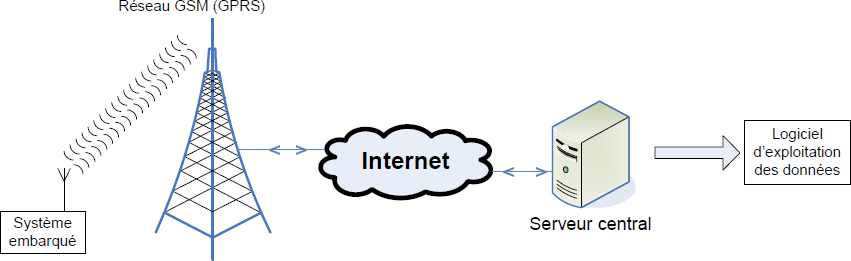
\includegraphics[width=17.463cm,height=5.345cm]{STB-img1.png} 

\textit{Connexion distante entre système embarqué et serveur central}

Le déploiement du système dans une station peut s’effectuer de deux
manières distinctes selon la nature de celle-ci : on parlera ainsi de
station filaire et de station non-filaire. Certaines stations pourront
éventuellement intégrer les deux moyens de communication et
d’alimentation, on parlera alors de station hybride.

 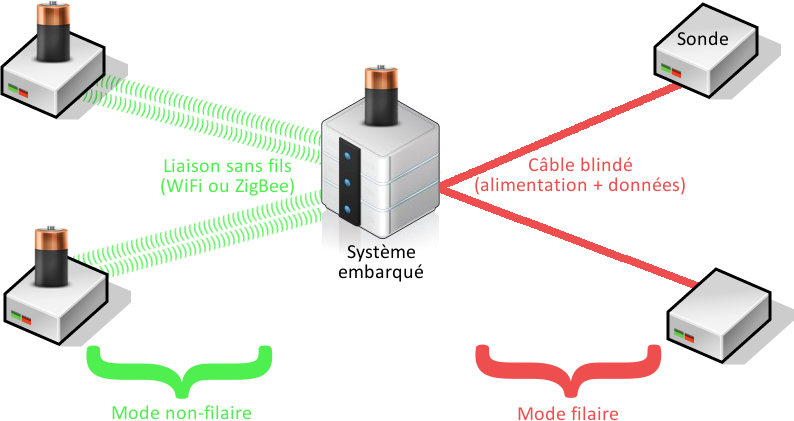
\includegraphics[width=15.505cm,height=8.229cm]{STB-img2.png}

\textit{Architecture d’un site hybride}

\subsection{Station filaire}

La connexion entre le système embarqué et les capteurs est physique
(câbles blindés), permettant l’échange bidirectionnel à la fois de
données, mais aussi à la distribution de l’alimentation depuis le
système central (contenant une batterie).

\subsection{Station non-filaire}

La connexion entre le système embarqué et les capteurs est
dématérialisée (ondes), à travers des technologies telles que ZigBee et
WiFi. La distinction sera faite en fonction de la nature de
l’environnement, le WiFi sera établit dès lors que le nombre de relais
ZigBee sera trop important où ils consommeront donc trop d’énergie (la
technologie ZigBee étant de plus faible portée). L’alimentation sera
elle déportée à chaque capteur où des piles longue durée assureront
l’autonomie de ces derniers.

\section{Bilan des améliorations}
Notre système doit améliorer certains points qui ne sont pour le moment
pas encore mis en place sur les sites. Il doit permettre une diminution
des coûts de trajet, réduire l’impact écologique des trajets des
opérations de livraison et de maintenances par la mise en place d’un
système d’aide à la décision et de gestion de trajets optimaux. Ceci
devra également être géré par la gestion de tous les sites en temps
réel basée sur un traitement en continue des données en provenance des
sites. Ce suivi pourra aboutir à une traçabilité des opérations et de
l’état des sites par l’utilisation de base de données stockées sur
serveurs qui pourra géré des règles d’anticipation des opérations de
maintenances et de livraison à réaliser. Ces règles pourront être
traitées par l’utilisation d’une intelligence artificielle.

Vu qu’aucun moyen de monitoring n’est disponible sur tous les sites à
observer, toutes ces améliorations seront à mettre en place sans avoir
de bases sur laquelle se fixer et se fier.

Après une étude approfondie, nous avons donc décidé d’utiliser divers
technologies pour mettre en place ce système de monitoring.

\subsection{Système à base de capteurs}
Pour le système de mesure des niveaux des cuves, notre choix se portera
sur des capteurs de niveau de type radar. Ce type de capteur est tout a
fait adapté pour fonctionner à des niveaux de pression et température
extrêmes. Ils sont également très précis avec des mesures ayant plus ou
moins 1 à 2 millimètres d’erreur. Ils sont également parfaitement
adaptés pour des mesures de matières à la fois liquides, solides et
pour n’importe quel type de matériaux. Le seul inconvénient sera la
mesure de produits plastiques, qui risque d’avoir plus d’imprécisions 
par l{\textquotesingle}absorption d’une parties des ondes émises pour
la mesure par ce genre de matériau.

Pour les secteurs à risques (cuves à essence, sites à taux de vandalisme
important), notre choix s’est tourné vers deux moyens techniques pour
en assurer la sécurité. Des capteurs de présence de type infra-rouges
seront utilisés. Ces capteurs peuvent détecter à distance tout intrus
voulant pénétrer sur les sites. Nous avons choisi d’associer un système
de caméras de surveillance pour identifier les éventuels malfrats. La
caméra de surveillance se lancera lorsqu’un capteur de présence aura
été déclenché. Le coût de cette seconde solution reste relativement
acceptable, mais elle utilisera une grande partie de la bande passante
du réseau.

Au niveau des mesures de pression, nous adopterons des mesures par des
baromètres numériques, pratiques pour traiter les informations et plus
résistants aux conditions extrêmes comparé aux baromètres analogiques

La mesure des températures se fera à l’aide de sonde en platine avec une
connectique réseau afin de gérer toutes les données récoltées par ce
genre de matériel. Ce type d’appareil de mesure est très adapté aux
conditions extrêmes et résiste à la majeur partie de produits
corrosifs.

L’ensemble des ces moyens technologiques seront installés en double afin
d’assurer un service en cas de panne d’un des capteurs par exemple.
Dans ce cas là, le second capteur installé prendra le relai. Cette
solution à moyen coût permettra de monitorer les sites avec des
défaillances matériels. Les maintenances pourront être planifiées de
manière plus optimisée.

\subsection{Système de géolocalisation}
Concernant les systèmes de localisation des véhicules des agents de
maintenances le meilleurs choix reste la technologie GPS. En effet sa
couverture planétaire et sa précision (15m-100m) en font un choix
parfait pour le cas général. En plus de ceci, cette technologie est
éprouvée, courante, standardisée et peu coûteuse.

Pour la localisation des sites, étant donné que dans le cas général les
sites sont statiques, il n’est donc pas nécessaire d’avoir une mise à
jour dynamique de cette position. C’est pourquoi la meilleurs solution
est une localisation unique (en se basant sur les données géographiques
ou sur une localisation GPS si il n’y a pas de données géographiques
disponibles). Cette localisation est ensuite stockée sur une base de
données centralisées. Ce sont ces données statiques qui sont transmises
aux agents de maintenances. Le système peut cependant aussi fonctionner
exceptionnellement en mode «dynamique» pour un site (site maritime
susceptible de se déplacer par exemple). La localisation se fera alors
par GPS.

\subsection{Système d’exploitation}
Le choix de l’OS se porte sur une solution spécifique répondant
parfaitement aux besoins. En effet, vu la simplicité des besoins, le
multi-tâche n’est pas nécessaire et la solution est de lire les valeurs
d’une série de capteurs puis de transmettre ces valeurs. Cette solution
permet ainsi de maintenir une totale maîtrise sur le système et de
permettre des évolutions futures.

\subsection{Apports énergétiques}
L’apport en énergie de tous les éléments du systèmes se fera de deux
façon différentes selon la facilité d’accès aux différents sites.

Pour les sites qui restent relativement accessible, notre choix se porte
vers une alimentation par batteries, qui seront remplacées lors des
opérations de maintenance ou bien rechargées si il y a un moyen de se
connecter sur secteur.

Pour les sites à grande difficulté d’accès, nous nous appuierons sur
l’utilisation de piles à hautes capacités. L’inconvénient majeur de
cette solution est le remplacement de celles-ci, car les opérations de
maintenance seront plus délicates à gérer en thermes d’optimisation 
des déplacements notamment.

\subsection{Communication}
Au niveau du type de connexion utillisé entre les différents sites et le
poste de contrôle, nous avons déterminé plusieurs solutions s’adaptant
au différentes scénarios possibles.

Pour les zones accessibles, une connexion filaire nous semble plus
adapté pour des coûts relativement raisonnables.

Pour les sites à grande difficulté d’accès, nous optons pour un système
de connexion Wi-Fi qui est beaucoup plus pratique en terme de
déploiement et de coût. On essaiera également de préserver
l’environnement par ce moyen. Si la distance entre les différents
capteurs et le système embarqué le permet (s’ils sont à une distance de
moins de 75m les uns des autres), il sera envisageable d’utiliser des
puces ZigBee à la place du Wi-Fi. Dans tous les cas, des tests de
qualité de réception seront effectués à l’installation.

Dans certaines situations, par exemple dans lieux soumis à de forts
champs électromagnétiques, on utilisera des connexions mixtes utilisant
les deux solutions précédentes pour palier aux perturbations des ondes.
\end{document}
